\chapter{Quality-Guided Path Unwrapping Algorithm}

As discussed in Section 2.3.2, the general algorithm which was used for phase unwrapping is the \textit{quality-guided path unwrapping algorithm} of Herraez, et al. which has a unique localized unwrapping path \cite{Herraez2002}.

All the figures and algorithms that will be shown in here are excerpts from their paper: ``Fast two-dimensional phase-unwrapping algorithm based on sorting by reliability following a noncontinuous path \cite{Herraez2002}."

The general flow of the algorithm will be illustrated in the following figures containing some numerical examples. Supposed we now have the computed reliability values for each pixel as shown in Fig. (a), an edge's reliability will be computed as the summation of the reliabilities the edge connects in Fig. (b) wherein the ones colored in red are vertically connected edges and colored in green are horizontally connected edges.

Unwrapping path is not defined by the reliability of the pixels but the reliability of the edges. The edges are stored in an array and sorted according to their reliability values. The edges with a higher reliabilities are unwrapped first.

\captionsetup[figure]{width=6in}
\begin{figure}[h!]
	\centering
	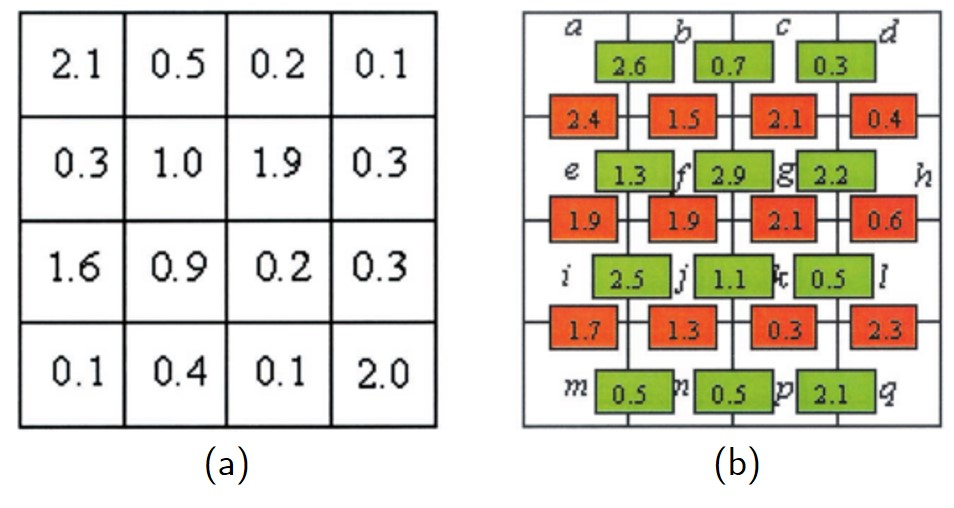
\includegraphics[width=0.7\textwidth]{figures/unwrap1.jpg}
	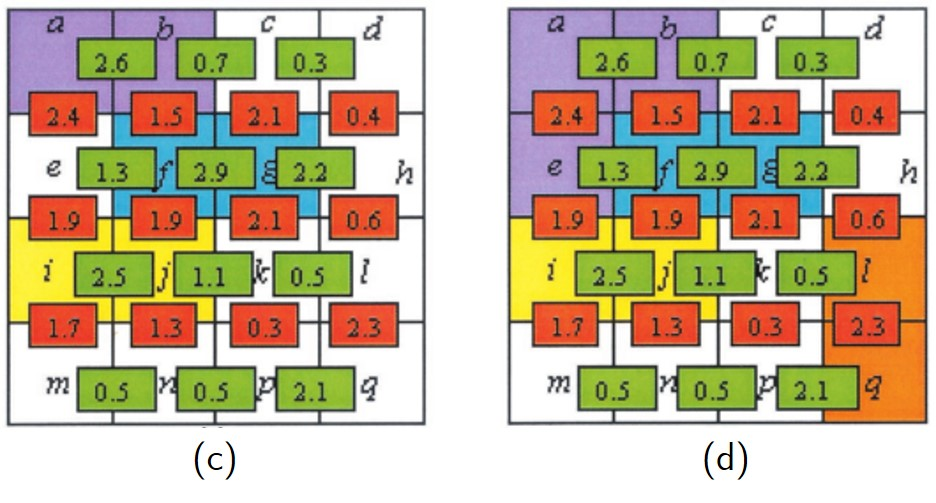
\includegraphics[width=0.7\textwidth]{figures/unwrap2.jpg}
	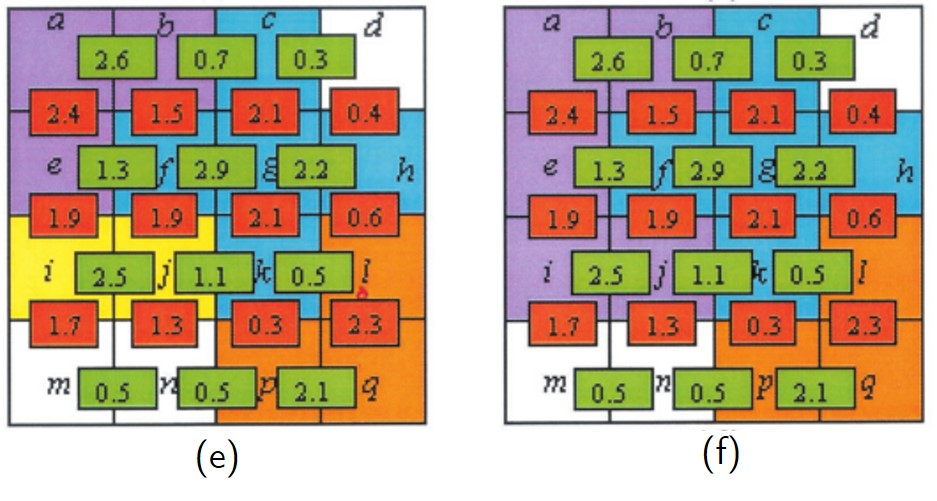
\includegraphics[width=0.7\textwidth]{figures/unwrap3.jpg}
	\caption[Unwrapping path]{Illustration of unwrapping path using numerical examples.}
	\label{fig:unwrap}
\end{figure}

For the unwrapping, pixels are initially considered as not belonging to any group. As seen in Fig. (c), the pixels with the highest reliability value (2.9) are \textit{f} and \textit{g} ($1^{st}$ group), thus they are unwrapped first with respect to each other. Pixels \textit{a} and \textit{b} are unwrapped next ($2^{nd}$ group) followed by pixels \textit{i} and \textit{j} ($3^{rd}$ group).

We see in Fig. (c) and (d) that the fourth highest value for an edge is shared by \textit{a} and \textit{e} and they should be unwrapped with respect to each other. However, \textit{a} is already unwrapped with respect to \textit{b} and has their own group. To unwrap pixel \textit{e}, the 2$\pi$ multiples required to be added/subtracted to unwrap pixel \textit{e} is calculated and added/subtracted to it. Pixels a, b, and e will now have the same group and is colored as one as shown in Fig. (d). 

\captionsetup[figure]{width=6in}
\begin{figure}[h!]
	\centering
	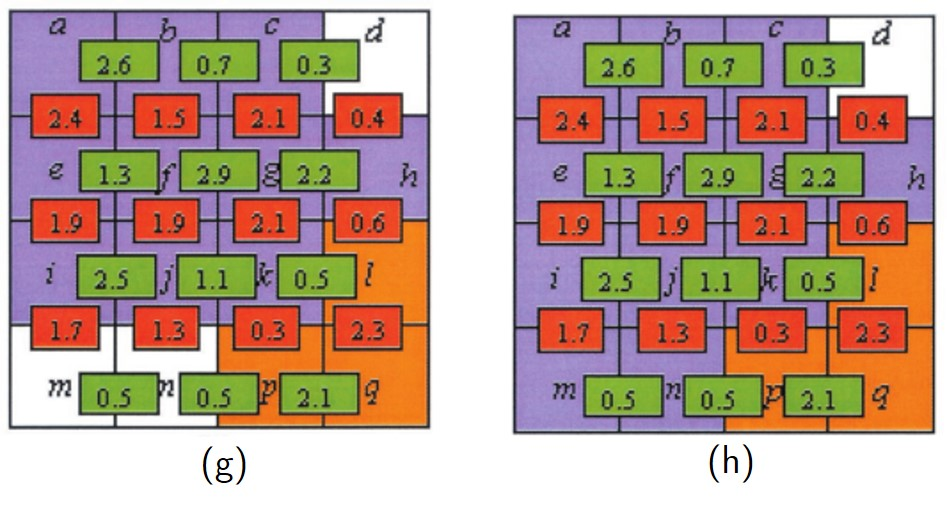
\includegraphics[width=0.7\textwidth]{figures/unwrap4.jpg}
	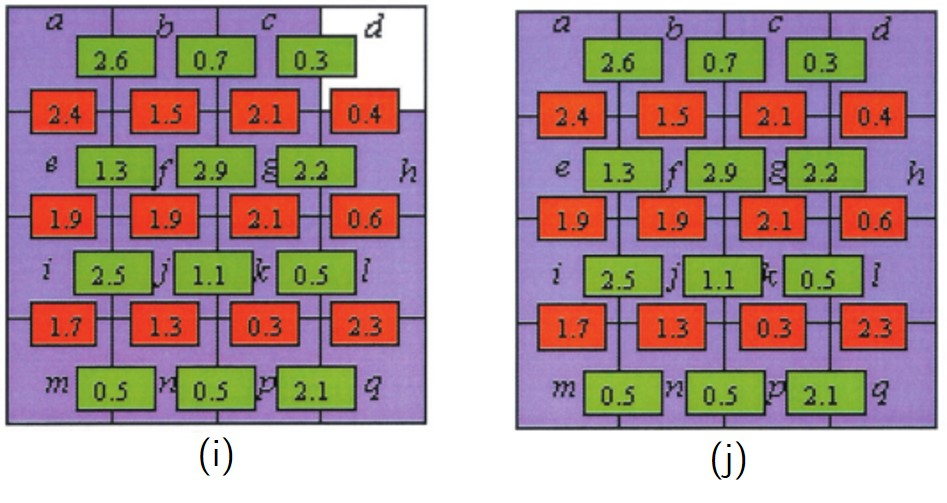
\includegraphics[width=0.7\textwidth]{figures/unwrap5.jpg}
	\caption[Continuation of unwrapping path]{Unwrapping path (\textit{continuation...}).}
	\label{fig:unwrap1}
\end{figure}

Fig. (e) and (f) illustrate the unwrapping of two groups with respect to each other with the first group consisting of pixels \textit{a}, \textit{b}, and \textit{e} and second group having pixels \textit{i} and \textit{j}. They are connected by a vertical edge and they share the next highest reliability value for an edge. Both groups are unwrapped with respect to each other. A pixel that belongs to the smaller group (less number of pixels) is unwrapped first with respect to any pixel in the larger group and the two groups will be joined together and colored as one as shown in Fig. (f). 

The algorithm will then proceed as shown in Fig. \ref{fig:unwrap1} until all pixels are unwrapped.

